\documentclass[a4paper]{article}

\usepackage[utf8]{inputenc}
\usepackage{indentfirst}
\usepackage{polski}
\usepackage{graphicx}
\usepackage{xcolor}
\usepackage{geometry}
\usepackage{float}


\newcommand\tab[1][1cm]{\hspace*{#1}}

\title{\textbf{Zraszacze Ogrodowe}}
\author{Jakub Grenda\\ Kamil Sztandur\\ Robert Odrowąż-Sypniewski}
\date{31/05/2020}
\begin{document}
\maketitle

\section{Cel Projektu.}
Celem naszego projektu było stworzenie programu, który pomagałby ogrodnikom w optymalnym rozstawieniu zraszaczy ogrodowych na terenie swojego trawnika. Program ten uwzględnia różne kształty terenu oraz obecne przeszkody na nim. Jego zadaniem jest rozstawienie odpowiedniej liczby czterech rodzajów zraszaczy ogrodowych tak, aby trawnik był podlany równomiernie na całej powierzchni. Program informuje użytkownika o ilości rozstawionych zraszaczy, ich koordynatach (oraz typach i kierunkach na konkretnych współrzędnych), średni stopień podlania całego trawnika oraz odchylenie standardowe od niego. \newline Najnowsza wersja aplikacji pozwala także na utworzenie specjalnej animacji, symulującej proces podlewania całego trawnika, która jest wyświetlana w czasie pracy programu, a następnie zapisywana w formacie GIF.
\newline

\begin{figure}[H]
    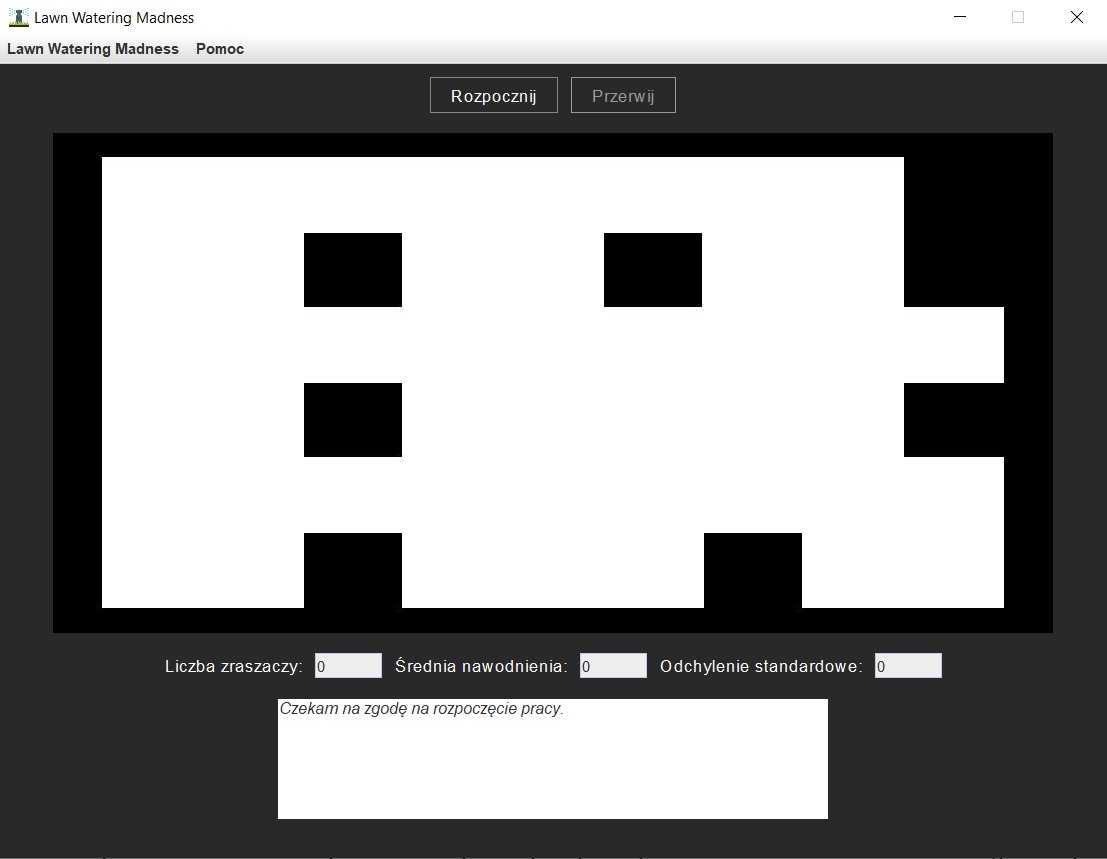
\includegraphics[width=11cm]{Podgląd.png}
    \centering
    \caption{Podgląd okna aplikacji}
\end{figure}

Użytkownik wprowadza do programu dane potrzebne do przeprowadzenia symulacji i pracy algorytmu rozstawiającego zraszacze. W czasie pracy programu użytkownik w specjalnym okienku jest cały czas informowany o procesach przebiegających w programie - bieżący etap pracy, dane właśnie rozstawionego zraszacza, numer aktualnie wyświetlanego cyklu (klatki), ewentualne komunikaty o problemach - oraz w specjalnych komórkach widoczna jest ilość rozstawionych przez algorytm zraszaczy, aktualna średnia arytmetyczna podlania całego trawnika oraz odchylenie standardowe od niej. Po zakończeniu pracy program generuje dane dot. rozstawienia zraszaczy, stanu trawnika oraz pozwalające na ponowne prześledzenie symulacji w razie potrzeby. Pomoc znajduje się w zakładce "Pomoc" na pasku menu w oknie aplikacji.

\section{Dane wejściowe programu.}
Po uruchomieniu aplikacji użytkownik wskazuje w oknie ustawień plik tekstowy na dysku, który zawiera kształt trawnika. Następnie wprowadza \textbf{czas trwania pojedynczych cykli}, które są jednostką czasu pracy naszych zraszaczy oraz okresem wyświetlania kolejnych klatek animacji. W przypadku potrzeby podania wartości niecałkowitej część ułamekową od jedności należy oddzielić \textbf{\underline{kropką}}. Kolejnym parametrem jest \textbf{ilość cykli}, które mają być symulowane (co jest równoznaczne z ilością klatek animacji). Każdy typ zraszacza potrzebuje inną ilość czasu dla swojego pełnego obrotu. Istnieje możliwość zaznaczenia opcji, aby program uwzględniał w symulacji \textbf{odbicia wytryskiwanej wody od powierzchni przeszkód}, co zwiększa wiarygodność wyników symulacji, ale również poważnie wydłuża czas pracy aplikacji i renderowania kolejnych klatek, co może spowodować opóźnienia wyświetlania kolejnych klatek. Aby rozwiązać ten problem, po zakończeniu pracy program generuje \textbf{animację GIF}, w której czas pomiędzy kolejnymi klatkami jest zawsze zgodny z czasem wprowadzonym przez użytkownika.

W kolejnych \textbf{40 liniach} wejściowego pliku tekstowego zawierających \textbf{80 znaków} danych oraz znak nowej linii określony jest kształt trawnika. Znaki danych to symbole '-' lub '*', gdzie '-' oznacza brak trawnika (lub przeszkodę) w danym punkcie natomiast '*' oznacza jego obecność. Każdy znak odpowiada kwadratowi o wymiarach 100x100 pixeli pliku wyjściowego jpg.

\newpage
\subsection*{Przykładowy plik wejściowy:}
\begin{verbatim}
--------------------------------------------------------------------------------
--------------------------------------------------------------------------------
----****************************************************************------------
----****************************************************************------------
----****************************************************************------------
----****************************************************************------------
----****************************************************************------------
----****************************************************************------------
----****************--------****************--------****************------------
----****************--------****************--------****************------------
----****************--------****************--------****************------------
----****************--------****************--------****************------------
----****************--------****************--------****************------------
----****************--------****************--------****************------------
----************************************************************************----
----************************************************************************----
----************************************************************************----
----************************************************************************----
----************************************************************************----
----************************************************************************----
----****************--------****************************************------------
----****************--------****************************************------------
----****************--------****************************************------------
----****************--------****************************************------------
----****************--------****************************************------------
----****************--------****************************************------------
----************************************************************************----
----************************************************************************----
----************************************************************************----
----************************************************************************----
----************************************************************************----
----************************************************************************----
----****************--------************************--------****************----
----****************--------************************--------****************----
----****************--------************************--------****************----
----****************--------************************--------****************----
----****************--------************************--------****************----
----****************--------************************--------****************----
--------------------------------------------------------------------------------
--------------------------------------------------------------------------------
\end{verbatim}
\newpage

\section{Przegląd sytuacji wyjątkowych opisywanych przez program.}
\subsection{Wejście.}
\begin{enumerate}
    \item Użytkownik podaje nieprawidłową wartość ilości lub długości cykli.
          \begin{itemize}
              \item Program wyświetla użytkownikowi okno z upomnieniem i informacją o prawidłowym uzupełnieniu parametrów.
              \item Po zamknięciu okienka z upomnieniem program wraca do okna ustawień.
          \end{itemize}
    \item Użytkownik zapomina podać plik tekstowy z trawnikiem.
          \begin{itemize}
              \item Program informuje użytkownika poprzez okienko o potrzebie podania pliku tekstowego.
              \item Po zamknięciu okienka z upomnieniem program wraca do okna ustawień.
          \end{itemize}
\end{enumerate}
\subsection{Przetwarzanie danych wprowadzonych przez użytkownika.}
\begin{enumerate}
    \item Po zaakceptowaniu podania pliku przez użytkownika, plik zostaje usunięty lub występują problemy z jego rozczytaniem. 
          \begin{itemize}
              \item Program wyświetla użytkownikowi komunikat o zaistniałym wariancie błędu.
              \item Program przerywa pracę, zachowując pliki konfiguracyjne dla przyszłej analizy.
          \end{itemize}
\end{enumerate}
\subsection{Renderowanie animacji.}
\begin{enumerate}
    \item Komputer użytkownika nie nadąża z renderowaniem kolejnych klatek animacji w porównaniu do czasu, jaką mu na to użytkownik wyznaczył.
          \begin{itemize}
              \item Program wyświetla komunikat o zaistniałym opóźnieniu w okienku logów.
              \item Program kontynuuje pracę.
          \end{itemize}
\end{enumerate}
\subsection{Ogólna praca programu.}
\begin{enumerate}
    \item W czasie pracy program z nieprzewidzianych przez programistów przyczyn napotkał krytyczny błąd i został zamknięty w czasie pracy.
          \begin{itemize}
              \item Program przerywa pracę.
              \item Dotychczasowe wyrenderowane klatki animacji znajdują się w katalogu zawierającym plik .jar w folderze resources w podfolderze temp.
          \end{itemize}
\end{enumerate}

\newpage
\section{Algorytm rozmieszczający zraszacze}
Działanie algorytmu rozpoczyna się od znalezienia i zaznaczenia w pomocniczej tablicy \textbf{int[][] edges} krawędzi trawnika. Dla zwiększenia wydajności algorytm na tym etapie operuje na danych o rozdzielczości pliku wejściowego tj. 80x40.

\begin{figure}[H]
    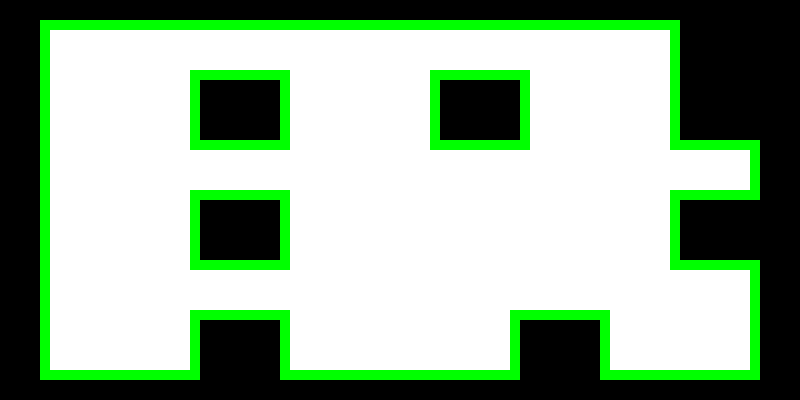
\includegraphics[width=10cm]{edges.png}
    \centering
    \caption{Odnalezione krawędzie trawnika}
\end{figure}

Po odnalezieniu krawędzie algorytm znajduje rogi o kącie \(90^{\circ}\) i umieszcza w nich zraszacze o takim zakresie podlewania. Następnie w na rogach o kącie \(270^{\circ}\) umieszczane są odpowiednie zraszacze. Jako ostatnie rozstawiane są zraszacze \(180^{\circ}\) wzdłuż prostych krawędzi trawnika.

\begin{figure}[H]
    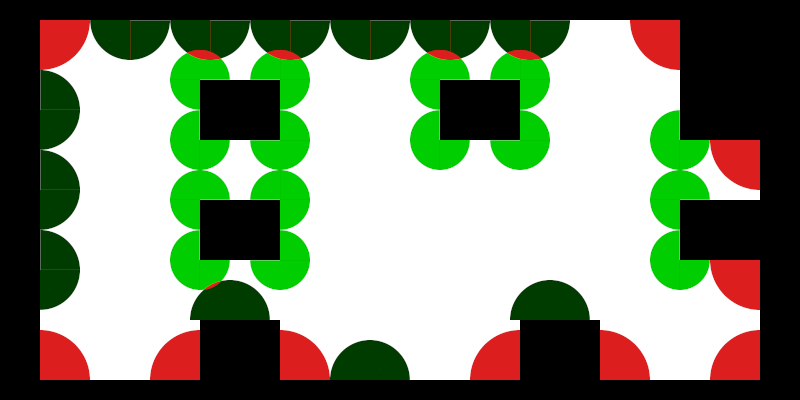
\includegraphics[width=10cm]{edge_sprinklers.png}
    \centering
    \caption{Trawnik po rozmieszczeniu krawędziowych zraszaczy}
\end{figure}

Następnie we wszystkich dotąd niepodlanych punktach ustawiane są zraszacze o zakresie pełnego okręgu rozpoczynając od lewego górnego rogu.

\begin{figure}[H]
    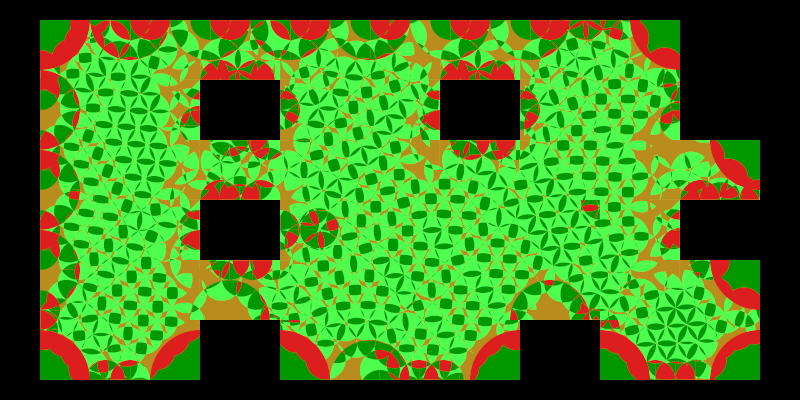
\includegraphics[width=10cm]{all_sprinklers.png}
    \centering
    \caption{Trawnik po wszystkich zraszaczy}
\end{figure}

W trakcie działania algorytmu kolejne zraszacze są dopisywane do ArrayListy zawierającej obiekty typu \textbf{Sprinkler} określające położenie (\textbf{koordynaty x, y}) zraszacza, jego \textbf{typ} (SprinkleType) oraz \textbf{kierunek} (Direction). Następnie program na jej podstawie rozpoczyna podlewanie trawnika oraz po ukończeniu pracy wypisuje ją do pliku tekstowego.

\newpage
\section{Opis funkcji udostępnianych przez program.}
Program dysponuje wachlarzem obiektów odpowiedzialnych za obsługę plików jpg, txt, gif, interfejsów graficznych Java Swing oraz potrzebnych funkcji matematycznych. 

\subsection{Config.}
\textbf{Najważniejszy obiekt informacyjny, którego wymagają prawie wszystkie obiekty w programie do prawidłowej pracy}. Tworzy on i zarządza plikiem konfiguracyjnym, który zawiera ścieżki, ustawienia użytkownika i inne ważne informacje dla prawie wszystkich pozostałych obiektów w programie. Obiekt zawiera wyłącznie funkcje statyczne.
\begin{enumerate}
    	\item \textbf{void createNewProperties()} - Funkcja tworząca plik konfiguracyjny typu Properties i przypisująca mu początkowe wartości.
    	\item \textbf{void saveToFile( Properties config )} - Funkcja zapisująca właściwości do pliku tekstowego (używana w createNewProperties).
    	\item \textbf{void deleteFile()} - Funkcja kasująca tekstowym plik konfiguracyjny z katologu programu.
    	\item \textbf{Properties readFile()} - Funkcja czytająca tekstowy plik konfiguracyjny i zwracająca obiekt typu Properties w nim zawarty.
    	\item \textbf{void set( String key, String value )} - Funkcja zapisująca lub nadpisująca pozycję ustawień w tekstowym pliku konfiguracyjnym.
    	\item \textbf{void get( String key )} - Funkcja pobierająca pozycję ustawień w tekstowym pliku konfiguracyjnym.
	\item \textbf{String getConfigFilename()} - Funkcja zwracająca nazwę tekstowego pliku konfiguracyjnego.
\end{enumerate}

\subsection{Sprinkler.}
\begin{figure}[H]
        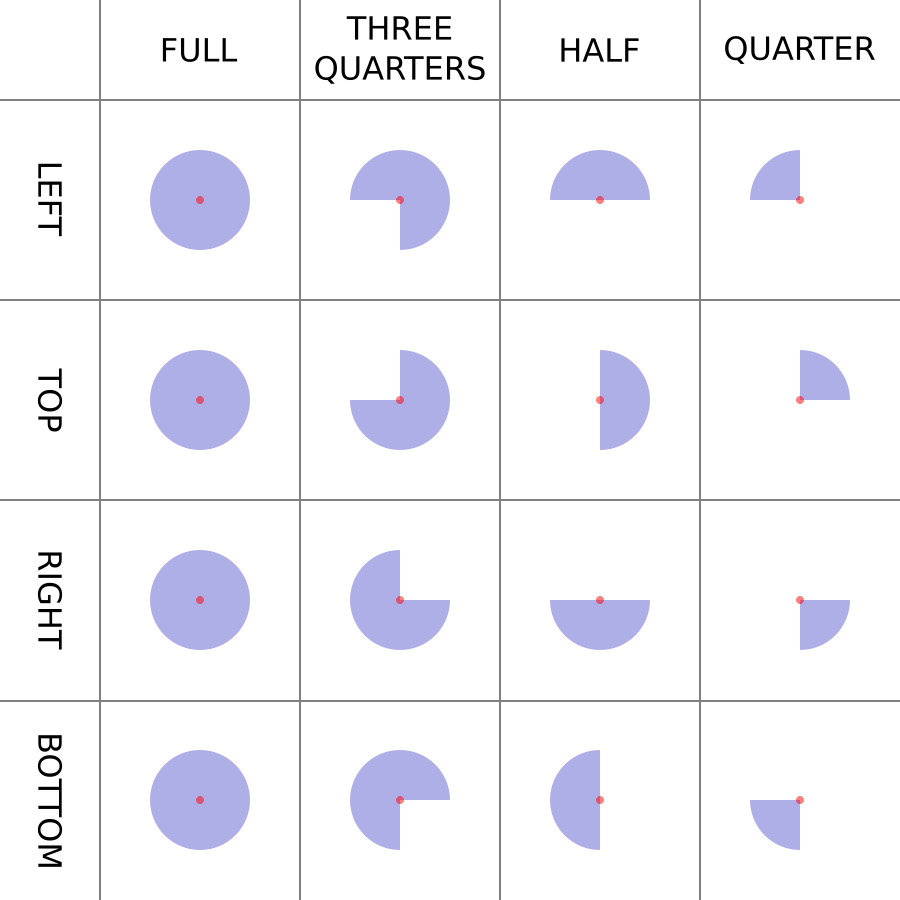
\includegraphics[width=10cm]{sprinklers.png}
        \centering
        \caption{\textit{Tabelka zraszaczy w postaci iloczynu kartezjańskiego ich typu i kierunku.}}
\end{figure}
Obiekt odpowiadający za zarządzanie zraszaczami, listą zraszaczy i zapewniający interfejs ułatwiający operacje na nich np. przy algorytmie.
\begin{enumerate}
    \item \textbf{Sprinklers} - Interfejs zawierający typy wyliczeniowe dla typów (SprinklerType) i kierunków (Direction) zraszaczy, przyporządkujący im wartości numeryczne oraz zawierający informacji o okresach obrotu i promieniach poszczególnych zraszaczy. 
	\item \textbf{Sprinkler} - Pojedynczy obiekt zraszacza. Przechowuje jego koordynaty (x, y), kierunek (Direction) oraz typ (SprinklerType)
	\item \textbf{SprinklersList} - Obiekt stanowiący listę zraszaczy oparty na ArrayList oraz opatrzony funkcją "add", która oprócz dodania zraszacza do ArrayListy wykonuje wszystkie inne potrzebne w programie akcje przy dodaniu zraszacza (np. wypisanie informacji o tym na interfejs graficzny). 
\end{enumerate}

\subsection{Stats.}
Obiekt zawierający wszystkie bardziej zaawansowane funkcje matematyczne dostosowane pod podawane im przez ten program obiekty głównie tablice dwuwymiarowe.
\begin{enumerate}
     \item \textbf{double avg ( int  lawn) } - Funkcja obliczająca średnią arytmetyczną z przyjmowanej tablicy dwuwymiarowej, zwraca -1 w przypadku wystąpienia wyjątku ArithmeticException.  Posługuje się wzorem:
          \[E_{(x)} = \frac{\sum_{i=1}^n x_i}{n}\]
          gdzie $x_i$ to kolejne wartości komórek tablicy, a $n$ to liczba wszystkich komórek.
	\item \textbf{double std\_deviation (int[][] lawn, double average)} - Funkcja obliczająca odchylenie standardowe z przyjętej tablicy dwuwymiarowej i średniej arytmetycznej.  Posługuje się wzorem:
          \[D(x) = \sqrt{\frac{\sum_{i=1}^n (x_i - E_{(x)})^2 }{n}}\]
          gdzie \(E_{(x)}\) to średnia arytmetyczna.
	\item \textbf{double std\_deviation(int[][] lawn) } - Przeciążenie funkcji obliczającej odchylenie standardowe z przyjętej tablicy dwuwymiarowej, ale przy braku średniej arytmetycznej.
\end{enumerate}


\subsection{WindowManager.}
Statyczny obiekt stanowiący ogólny podręczny menedżer okien interfejsu graficznego użytkownika
\begin{enumerate}
    \item \textbf{void waitUntilClosed( JFrame Window )} - statyczna funkcja, która każe bieżącemu wątkowi czekać dopóki użytkownik nie zamknie okna interfejsu graficznego Java Swing podanego jako parametr.
\end{enumerate}

\subsection{WindowMenuBar.}
Obiekt paska menu w oknach interfejsu graficznego na bazie Java Swing.
\begin{enumerate}
    	\item \textbf{WindowMenuBar} - Interfejs graficzny panelu menu w oknie programu wraz z całą logiką i nasłuchiwaczami.
	\item \textbf{InfoWindow} - Niepubliczna klasa przechowująca w obiekcie wyskakujące okna z informacjami po wybraniu którejkolwiek z opcji w pasku menu. Jako argument przyjmuje tytuł okna, informacja która ma zostać wypisana w oknie oraz ścieżkę do obrazka przykładowego (może być null - wtedy nie będzie obrazka). 
\end{enumerate}


\subsection{SettingsWindow.}
Obiekt przechowujący okno ustawień wyskakujące na początku programu. Współpracuje z obiektem Settings, która obsługuje nasłuchiwacze i komunikuje się z plikami konfiguracyjnymi. Zawiera szereg funkcji renderujących poszczególne panele okna.

\subsection{Settings.}
Obiekt przechowujący logikę okna ustawień SettingsWindow. Obsługuje nasłuchiwacze, weryfikuje poprawność i zapisuje wprowadzone przez użytkownika dane do pliku konfiguracyjnego config.txt.
\begin{enumerate}
    	\item \textbf{void actionPerformed( ActionEvent event )} - Funkcja obsługująca naciśnięte przez użytkownika przyciski w oknie ustawień.
    	\item \textbf{void itemStateChanged( ItemEvent e )} - Funkcja obsługująca zaptaszkowanie checkboxa przez użytkownika.
    	\item \textbf{private void modifyField( JTextField field, int mode )} - Funkcja modyfikowania pola w oknie z ilością cykli za pomocą przycisków wokół.
    	\item \textbf{private void getFile()} - Funkcja otwierająca okno wyszukiwarki plików w systemie operacyjnym, pozwalająca w wygodny sposób wskazać użytkownikowi plik wejściowy.
\end{enumerate}

\subsection{ResultWindow.}
Obiekt przechowujący okno finałowe wyskakujące na zakończenie pracy programu, informująca o jego przebiegu i wyniku. Zawiera szereg funkcji renderujących poszczególne panele okna.

\subsection{Result.}
Obiekt przechowujący logikę okna finałowego ResultWindow. Obsługuje nasłuchiwacz kliknięcia przycisku przez użytkownika.
\begin{enumerate}
    	\item \textbf{void actionPerformed( ActionEvent event )} - Funkcja obsługująca naciśnięte przez użytkownika przyciski w oknie finałowym.
\end{enumerate}

\subsection{Output.}
Obiekt obsługujący całe potrzebne wyjście w programie.
\begin{enumerate}
    	\item \textbf{void export\_jpg(int[][], double average, double stdv, String img\_filename )}  - Funkcja eksportująca obrazek jpg z tablicy dwuwymiarowej, korzystająca z obiektu tłumaczącego kolory HSV na RGB i kolorująca w oparciu o średnią arytmetyczną i odchylenie standardowe, a następnie tworząca obrazek jpg o podanej nazwie.
\newline Każdy pixel trawnika jest kolorowany w oparciu o wartość odpowiadającej mu komórki w tablicy 2D. Sposób kolorowania jest zależny od wyliczonej średniej arytmetycznej oraz odchylenia standardowego \textit{(Rysunek 2.)}.

\begin{figure}[H]
    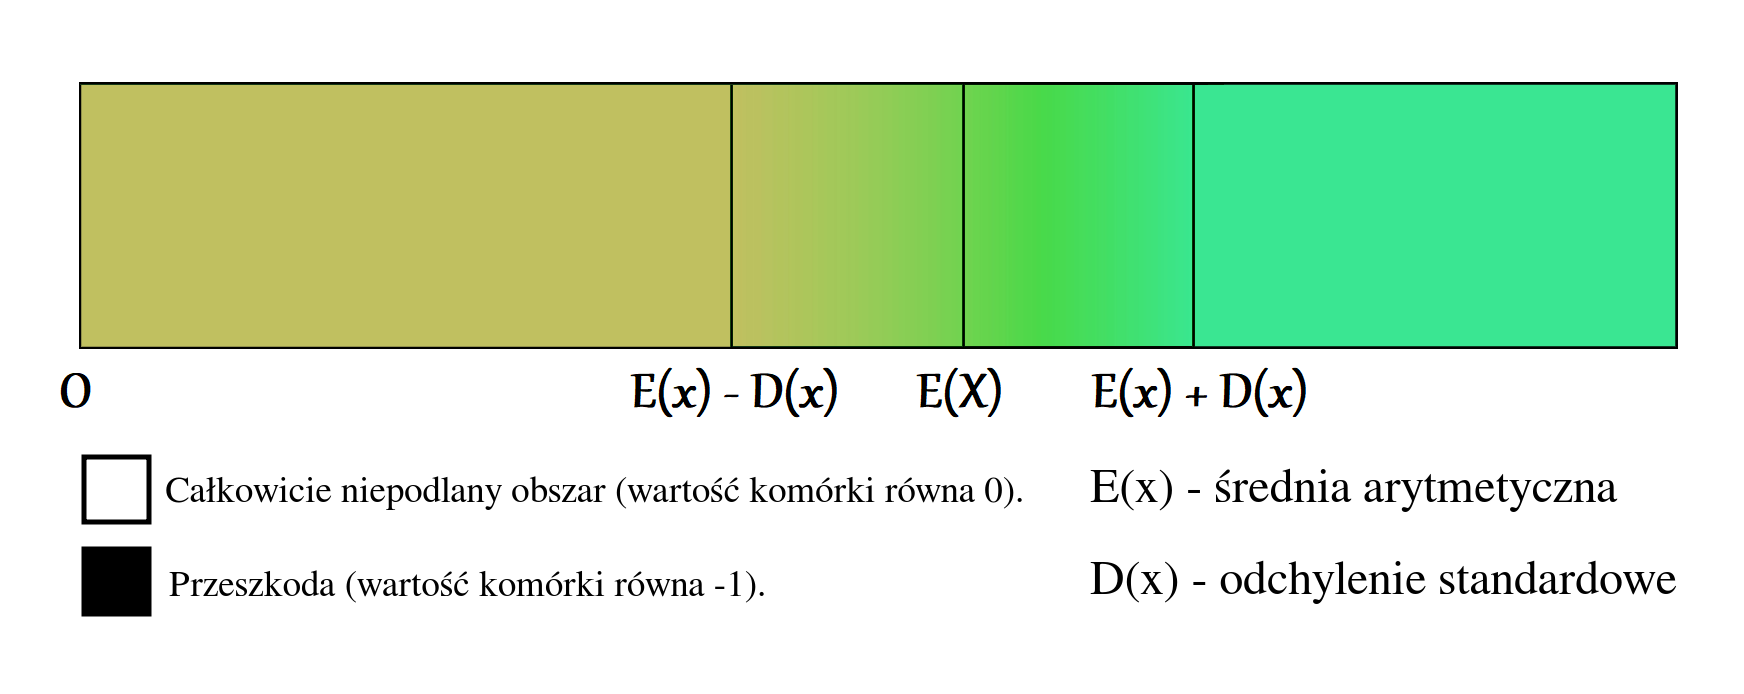
\includegraphics[width=10cm]{kolory.png}
    \centering
    \caption{\textit{Metoda kolorowania komórek}}
\end{figure}

\begin{itemize}
    \item Wartości spomiędzy przedziału (E(x) – D(x), E(x) + D(x)) są gradientem zieleni i oznaczają prawidłowe wartości nawodnienia trawnika.
    \item Wartości poniżej dolnej granicy są koloru zgniło-żółtego i oznaczają niedostatecznie podlane komórki w porównaniu do całości.
    \item Wartości powyżej górnej granicy są koloru mokrej zieleni i oznaczają zbytnio podlane komórki w porównaniu do całości.
\end{itemize}
    	\item \textbf{void export\_txt(ArrayList$\langle Sprinkler \rangle$ sprinklers\_list)} - Funkcja eksportująca plik tekstowy "koordynaty.txt" z listą zraszaczy podaną jako parametr.
\begin{figure}[H]
        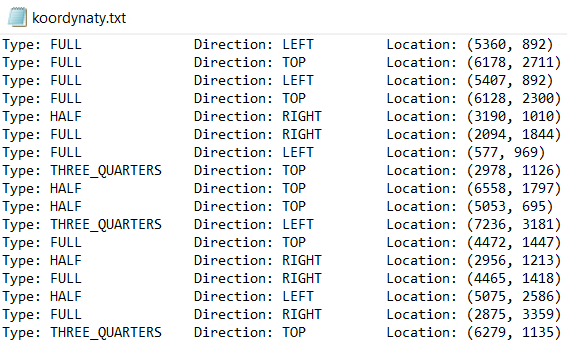
\includegraphics[width=10cm]{koordynaty.png}
        \centering
        \caption{\textit{Przykładowy tekstowy plik wyjściowy.}}
\end{figure}
    	\item \textbf{private void writeLine( FileOutputStream stream, String lineToWrite )} - Funkcja prywatna pomocna przy wypisywaniu listy do pliku.
    	\item \textbf{boolean create\_dir(String dirname)} - Funkcja tworząca folder o podanej nazwie (jeżeli jeszcze taki nie istnieje) i zwracająca true, jeżeli udało się utworzyć folder.
\end{enumerate}

\subsection{MainWindowEvents.}
Obiekt obsługujący logikę głównego okna interfejsu graficznego, gdzie wyświetlana jest animacja, logi programu oraz wartości liczbowe w programie. Użytkownik może rozpocząć, wstrzymywać i wznawiać pracę programu z tego poziomu. To stąd startuje wątek animacji. Obsługuje nasłuchiwacze MainWindow.
\begin{enumerate}
    	\item \textbf{void actionPerformed( ActionEvent event )} - Funkcja obsługująca naciśnięte przez użytkownika przyciski w oknie. Pierwsze uruchomienie animacji z komendy "Rozpocznij" rozpoczyna rozstawianie zraszaczy przez algorytm, a następnie startuje wątek animacji. Przyciski "Wznów" i "Zatrzymaj" pozwalają na zarządzanie programem.
\end{enumerate}

\subsection{MainWindow.}
Obiekt przechowujący główne okno interfejsu graficznego, gdzie wyświetlana jest animacja, logi programu oraz wartości liczbowe w programie. Zawiera nasłuchiwacze, które są obsługiwane przez MainWindowEvents, funkcje renderujące kolejne panele w oknie oraz funkcje pomocnicze do modyfikowania wartości znajdujących się w oknie (średnia, odchylenie, ilość zraszaczy, dodawanie logów programu).
\begin{enumerate}
    	\item \textbf{void printNewAction(String action)} - Funkcja dopisująca do logów w oknie przekazaną jako parametr typu String akcję. 
    	\item \textbf{void updateSprinklerAmount(int n)} - Funkcja ustawiająca liczbę przekazaną poprzez parametr jako wyświetlaną ilość zraszaczy w oknie.
    	\item \textbf{void updateAverage()} - Funkcja aktualizująca wyświetlaną w oknie średnią arytmetyczną z tablicy dwuwymiarowej trawnika, korzystająca z obiektu Lawn, którego wskaźnik jest zapisany w tym obiekcie MainWindow.
    	\item \textbf{void updateStdv()} - Funkcja aktualizująca wyświetlane w oknie odchylenie standardowe z tablicy dwuwymiarowej trawnika, korzystająca z obiektu Lawn, którego wskaźnik jest zapisany w tym obiekcie MainWindow. Warto poprzedzić tę funkcję powyższą funkcją updateAverage podczas użycia, ponieważ zakłada ona aktualność średniej arytmetycznej.
\end{enumerate}

\subsection{Lawn.}
Obiekt trawnika, zawierający tablicę dwuwymiarową 4000x8000 jego stanu, 40x80 jego kształtu (na potrzeby algorytmu) oraz zmniejszonych rozmiarów kopię 400x800 na potrzeby wyświetlania animacji ze względu na problemy wydajnościowe przy renderingu animacji 8k. Oprócz tego przechowuje także stałe wielkości poszczególnych tablic oraz średnią i odchylenie standardowe z trawnika 4000x8000.
\newline Obiekt inicjalizuje się bez żadnych parametrów. Korzysta on informacji pliku config.exe zmodyfikowanego przez obiekt Settings. 
\begin{enumerate}
    	\item \textbf{void parseShape()} - Tworząca tablicę dwuwymiarową 40x80 w obiekcie Lawn, będąca odwzorowaniem kształtu trawnika. Potrzebne do algorytmu. 
    	\item \textbf{void upscaleShape()} - Funkcja skalująca tablicę dwuwymiarową 40x80 kształtu trawnika na rzeczywistą wielkość 4000x8000, na której będzie pracować program.
    	\item \textbf{void update\_gif\_lawn()} - Funkcja aktualizująca tablicę 400x800 trawnika dla animacji na podstawie oryginalnej tablicy 4000x8000. Wykorzystuje do algorytm dzielący oryginalną tablicę na pomniejsze tablice 10x10 i liczący średnią z ich środkowych i narożnikowych komórek. Następnie przypisuje tę średnią jednej komórce odpowiadającej im położeniem na tablicy 400x800. W ten sposób ta komórka w przybliżony sposób reprezentuje tamtą tablicę 10x10 w optymalny sposób, ponieważ liczenie średniej z całej tablicy 10x10 zajmuje zbyt dużo czasu jak na trwającą animację.

\begin{figure}[H]
    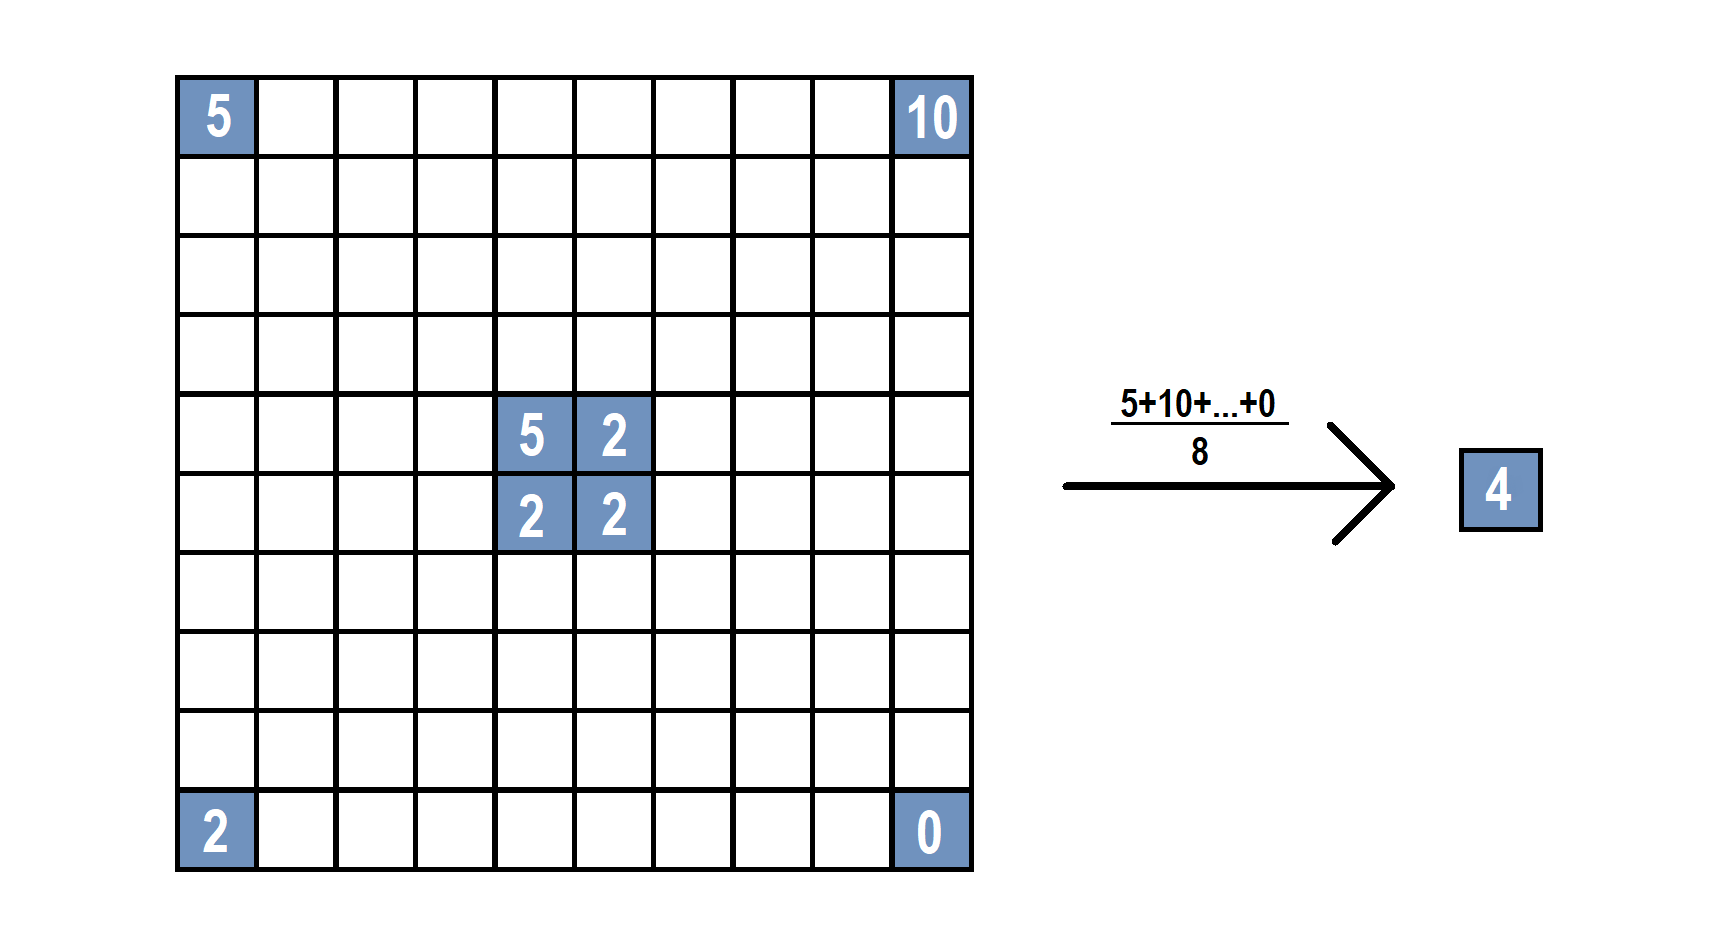
\includegraphics[width=10cm]{parse_gif.png}
    \centering
    \caption{Sposób skalowania dużej tablicy trawnika na mniejszą, używaną do wyświetlania animacji.}
\end{figure}

    	\item \textbf{void updateAverage()} - Funkcja aktualizująca przechowywaną w tym obiekcie średnią arytmetyczną z tablicy dwuwymiarowej trawnika, korzystająca z obiektu Stats zawierającego potrzebne obliczenia matematyczne.
    	\item \textbf{void updateStdv()} - Funkcja aktualizująca przechowywane w tym obiekcie odchylenie standardowe z tablicy dwuwymiarowej trawnika, korzystająca z obiektu Stats zawierającego potrzebne obliczenia matematyczne. Warto poprzedzić tę funkcję powyższą funkcją updateAverage podczas użycia, ponieważ zakłada ona aktualność średniej arytmetycznej.
\end{enumerate}

\subsection{HSVtoRGB.}
Statyczny obiekt tłumaczący wartości HSV na RGB.
\begin{enumerate}
    	\item \textbf{int[] calc( double h, double s, double v )} - Funkcja tłumacząca wartości HSV na RGB i zwracająca jednowymiarową tablicę. Parametr h przyjmuje wartości z przedziału [0, 360], parametr s z przedziału [0, 1] oraz parametr v z przedziału [0, 1].
\end{enumerate}

\subsection{GifSequenceWriter.}
Biblioteka zawierająca metody tworzące animację GIF z utworzonych klatek w trakcie pracy programu. Autorem tej biblioteki jest twórca strony \emph{https://memorynotfound.com}. Zamieścił ją tam do pobrania i użytku publicznego.

\subsection{GIF.}
Obiekt przechowujący wątek odpowiedzialny za wyświetlanie animacji w oknie aplikacji i tworzenie kolejnych klatek animacji, zawierający również narzędzia do utworzenia pliku GIF na końcu pracy programu.
\begin{enumerate}
    	\item \textbf{void run()} - Funkcja główna wątku animacji, odpowiedzialna za jej prawidłową pracę i wyświetlanie. Może być wstrzymany z poziomu interfejsu graficznego okna głównego MainWindow.
    	\item \textbf{void generateGIF()} - Funkcja tworząca animację GIF z klatek utworzonych w czasie pracy wątku animacji. Korzysta z obiektów GifSequenceWriter oraz HSVtoRGB.
    	\item \textbf{void createWorkdir()} - Funkcja tworząca tymczasowy folder roboczy, w której program zapisuje kolejne wyrenderowane klatki animacji.
    	\item \textbf{void cleanWorkdir()} - Funkcja kasująca tymczasowy folder roboczy, w której program zapisuje kolejne wyrenderowane klatki animacji.
    	\item \textbf{void drawCircles()} - Funkcja wprowadzająca zmiany w wyglądzie trawnika wywoływana przy każdej kolejnej klatce animacji. Korzysta z obiektu Drawer do wprowadzania zmian oraz obiektu SprinklerList zawierającego listę rozstawionych zraszaczy.
\end{enumerate}

\subsection{ErrorWindowEvents oraz Error.}
Klasa zawierająca obiekt obsługujący nasłuchiwacze akcji na interfejsie graficznym okna wyskakującego błędu ErrorWindow. Zawiera również obiekt Error zawierający metodę do uruchamiania takiego okna i zaleca się uruchamianie tego okna tylko za pomocą tej metody.
\begin{enumerate}
    	\item \textbf{void popErrorWindow(String error\_message, int mode, boolean wait )} - Statyczna funkcja w obiekcie Error wyświetlająca na ekran okno z powiadomieniem o błędzie. Przyjmuje jako parametry treść wiadomości o błędzie, informację w jakim trybie wyskakuje to okno (JFrame.DISPOSE\_ON\_CLOSE albo JFrame.EXIT\_ON\_CLOSE) oraz boolowską wartość, czy program na czekać aż okno zostanie zamknięte przez użytkownika.
\end{enumerate}

\subsection{ErrorWindow.}
Obiekt przechowujący okno błędu wyskakujące za wywołaniem metody popErrorWindow z obiektu Error, informująca o przyczynie błędu i decydująca o dalszej pracy programu. Zawiera szereg funkcji renderujących poszczególne panele okna.

\subsection{Drawer.}
Klasa odpowiedzialny za wprowadzanie zmian na tablicy dwuwymiarowej trawnika poprzez "rysowanie" kół zraszaczy, podwyższając wartości obejmowanych komórek o 1. Potrzebuje tablicy dwuwymiarowej trawnika oraz obiektu Sprinkler, na podstawie którego wprowadzi zmiany w tablicy. Zalecane jest zapoznanie się z interfejsem Sprinklers i numerycznymi odpowiednikami typów i kierunków zraszaczy.
\begin{enumerate}
    	\item \textbf{boolean contains\_quarter( int quarter, SprinklerType type, Direction direction )} - Funkcja sprawdzająca, czy przekazana ćwiartka koła znajdzie się w obrębie aktualnie rysowanego zraszacza. 
    	\item \textbf{void fix\_value\_artefacts( int[][] tab, Sprinkler sprinkler, int r )} - Funkcja przyjmująca tablicę dwuwymiarową trawnika, zraszacz oraz promień zraszacza, poprawiająca artefakty takie jak komórki, które przypadkiem powiększyły się kilka razy przy rysowaniu lub zostały pominięte.
    	\item \textbf{void draw\_circle\_with\_reflections( int[][] tab, Sprinkler sprinkler)} - Funkcja rysująca na przyjętej tablicy dwuwymiarowej trawnika zraszacz przyjęty jako drugi parametr z uwzględnieniem odbić wody od przeszkód (znacznie pogorsza wydajność programu).
    	\item \textbf{void draw\_circle\_without\_reflections( int[][] tab, Sprinkler sprinkler)} - Funkcja rysująca na przyjętej tablicy dwuwymiarowej trawnika zraszacz przyjęty jako drugi parametr z pominięciem odbić wody od przeszkód.
\end{enumerate}

\subsection{Algorithm.}
Obiekt odpowiedzialny za rozstawienie zraszaczy na trawniku. Potrzebuje obiektu interfejsu graficznego okna, na którym wyświetla się animacja, obiektu Lawn trawnika oraz listy zraszaczy w obiekcie SprinklersList.
\begin{enumerate}
    	\item \textbf{void setSprinklers()} - Funkcja główna algorytmu rozstawiająca zraszacze.
\end{enumerate}

\end{document}
